\documentclass[conference]{IEEEtran}

\usepackage[spanish]{babel}
\usepackage{amsmath,amssymb,amsfonts,amsthm}
\usepackage{graphicx}
\usepackage[utf8]{inputenc} % Caracteres en Español (Acentos, ñs)
\usepackage{url} % ACENTOS
\usepackage{hyperref} % Referencias
\usepackage{float}
\usepackage[spanish]{csquotes}
\usepackage{caption}
\captionsetup{skip=0pt} 
\usepackage[font=medium,skip=15pt]{caption} 

\usepackage{etoolbox}
\makeatletter
\patchcmd{\frontmatter@RRAP@format}{(}{}{}{}
\patchcmd{\frontmatter@RRAP@format}{)}{}{}{}
\makeatother


\usepackage[backend=bibtex,sorting=none]{biblatex}
\addbibresource{references.bib}

\usepackage{datetime}
\newdateformat{specialdate}{\twodigit{\THEDAY}-\twodigit{\THEMONTH}-\THEYEAR}
\date{\specialdate\today}

\renewcommand\spanishtablename{Tabla}
\renewcommand\spanishfigurename{Figura}

\begin{document}

\title{Reporte Proyecto Individual Unidad 3 \\ Aplicación Móvil Generadora de Sopa de Letras en PDF}

\author{\IEEEauthorblockN{Erika Daniela Mallozzi Martínez}
\IEEEauthorblockA{\IEEEauthorrefmark{} Ingeniería en Tecnologías de la Información\\
Universidad Politécnica de Victoria}
}

\maketitle

\begin{abstract} 
El presente proyecto describe el desarrollo de una aplicación móvil que permite generar sopas de letras personalizadas en formato PDF. Los usuarios pueden ingresar palabras clave de su preferencia y cuantas quiera, así como un número de páginas para crear su sopa de letras, la cual se genera en formato PDF para ser descargada o visualizada. Esta aplicación fue desarrollada utilizando Java y el IDE de Android Studio, y busca proporcionar una herramienta interactiva para generar este tipo de pasatiempos.

\end{abstract}

\section{Introducción}

Las sopas de letras son un juego de palabras y rompecabezas ampliamente conocido, que consiste en buscar y encontrar palabras escondidas en una cuadrícula de letras. Su origen exacto es incierto, pero existen antecedentes similares, como los cuadrados mágicos
creados en la Edad Media en Europa. En su forma moderna, la sopa de letras fue popularizada en Estados Unidos durante la década de 1960, atribuida a Norman E. Gibat, quien las utilizó para atraer lectores a su publicación *Selenby Digest*. En España, se reconoce a Pedro Ocón como un creador prolífico de pasatiempos, incluyendo este famoso juego \cite{milenio}.

Este pasatiempo ha evolucionado desde simples hojas de papel hasta aplicaciones digitales y herramientas interactivas, convirtiéndose en una actividad recreativa y educativa ampliamente utilizada.

Además, las sopas de letras tienen beneficios importantes para la salud y el aprendizaje. Expertos aseguran que mejoran la agudeza mental, la memoria, la concentración y el vocabulario. También alivian el estrés y fomentan el aprendizaje de nuevos idiomas, convirtiéndose en una herramienta versátil para todas las edades \cite{lanacion}.


Las aplicaciones móviles han ganado una gran popularidad en los últimos años debido a su accesibilidad y funcionalidad. Este proyecto tiene como objetivo el desarrollo de una aplicación móvil para generar  \textit{sopas de letras} en formato PDF, un juego educativo muy popular que puede ser personalizado para diversos contextos, desde la educación hasta el entretenimiento.

El desarrollo de esta aplicación fue realizado en lenguaje Java y el IDE de Android Studio, con la finalidad de crear una experiencia intuitiva para el usuario. La principal funcionalidad de la aplicación es permitir al usuario ingresar palabras clave y generar una sopa de letras con ellas, la cual se puede exportar a un archivo PDF para su descarga o impresión.

Esta aplicación móvil es de gran ayuda para la fácil y sencilla creación de material didáctico ya sea para enseñanza o pasatiempo, las ventajas de esta aplicación generadora de sopa de letras es que el usuario puede ingresar las palabras de su agrado y tambien seleccionará el numero de páginas que tendrá su sopa de letras, cada una de estas será diferente pero contendrá las mismas palabras que seleccionó dicho usuario. 


\section{Desarrollo Experimental}
El desarrollo de la aplicación se llevó a cabo en el entorno de desarrollo integrado (IDE) Android Studio \cite{androidstudio}, seleccionado por su capacidad para facilitar la creación de aplicaciones Android mediante herramientas avanzadas, integración con emuladores y compatibilidad con bibliotecas externas. La estructura del proyecto se diseñó siguiendo una arquitectura modular para mantener la escalabilidad y facilidad de mantenimiento del código.

La finalidad principal de la aplicación es permitir a los usuarios generar sopas de letras personalizadas en formato PDF, abordando tres funcionalidades principales: la entrada de palabras clave, la configuración del número de páginas y la creación y visualización del archivo PDF resultante.

\subsection{Interfaz de Usuario} El diseño de la interfaz de usuario (UI) sigue principios de usabilidad y simplicidad. Para ello, se utilizó un GridLayout en combinación con elementos de diseño nativo de Android, como campos de texto, botones y vistas. La interfaz consta de:

\begin{itemize}
    \item Campo de entrada para palabras clave: Permite al usuario ingresar las palabras que aparecerán en la sopa de letras.

    \item Campo de configuración para el número de páginas: Proporciona flexibilidad en el diseño al permitir al usuario definir la cantidad de páginas que desea generar.

    \item Botón de generación de PDF: Ejecuta el proceso de creación del archivo PDF, integrando las palabras clave y parámetros definidos.

    \item Botón de visualización del PDF: Muestra el archivo generado directamente en la aplicación, utilizando una vista compatible con documentos PDF.
\end{itemize}

Se implementó un diseño responsivo para asegurar que la aplicación sea accesible y funcional en diferentes tamaños de pantalla.

\subsection{Generación del PDF}
La generación de los archivos PDF es uno de los componentes clave del proyecto, lograda mediante la integración de la biblioteca iText \cite{itextpdf}, esta fue utilizada debido a su robustez y facilidad de integración en aplicaciones móviles. 
Una vez que el usuario ingresa las palabras y el número de páginas, la aplicación genera la sopa de letras en un formato predefinido, utilizando la biblioteca iText para la creación del archivo PDF. El archivo generado tiene opción de abrir y visualizar desde la misma aplicación para una mejor experiencia de usuario.
El proceso de generación incluye:
\begin{itemize}
    \item Construcción de la cuadrícula de la sopa de letras: Las palabras clave ingresadas se distribuyen de manera aleatoria dentro de una matriz. Las celdas vacías se completan con letras generadas aleatoriamente para garantizar la integridad visual del rompecabezas.

    \item Diseño del contenido PDF: Utilizando las herramientas proporcionadas por iText, se establece un diseño consistente para cada página, asegurando que las palabras y la cuadrícula se representen claramente.

    \item Creación del archivo PDF: Se compila el contenido generado en un archivo PDF estructurado, listo para visualizarse o compartirse.
\end{itemize}





\subsection{Tecnologías Utilizadas}
El proyecto se desarrolló en Java, aprovechando su robustez y extensas bibliotecas para el desarrollo de aplicaciones móviles. Las tecnologías y principios clave incluyen:
\begin{itemize}
      \item Biblioteca iText: Utilizada para manejar la creación de documentos PDF, con características específicas para agregar textos dinámicos, imágenes y estructuras de tablas.

       \item GridLayout: Implementado para organizar y renderizar las letras de la sopa de manera visualmente atractiva.

      \item Modelo Vista-Controlador (MVC): Adoptado para mantener una clara separación entre la lógica de negocio, la presentación y el control de eventos.

      \item Validación de entrada del usuario: Mecanismos que aseguran que las palabras ingresadas no excedan los límites permitidos y que el número de páginas sea razonable, evitando errores durante la generación del archivo.
\end{itemize}


\section{Resultados}

En esta sección se describen las principales características y funcionalidades de la \textbf{\textit{Aplicación Móvil Generadora de Sopa de Letras en PDF}} desarrollada. 
La aplicación fue evaluada en diferentes dispositivos Android, mostrando una generación eficiente de sopas de letras en formato PDF. Al ejecutar la aplicación, tras ingresar los datos necesarios, el archivo PDF es generado y descargado correctamente.

La funcionalidad de selección de palabras y la visualización de la sopa de letras fueron probadas con diferentes combinaciones de palabras, para con esto validar resultados no deseados como la escritura de palabras en el teclado con espacios o números, mostrando que el sistema maneja bien distintos tipos de entradas.

En la Figura \ref{fig:1}, se presenta la interfaz inicial de la aplicación. Esta es la pantalla donde el usuario ingresa las palabras para la sopa de letras. Se diseñó esta interfaz amigable para que fuera sencilla de entender por cualquier persona. 

Describiendo lo que se aprecia visualmente, se presenta el tirulo de la aplicación, una breve instrucción para el usuario, y dos campos para ingresar texto, en el primero el usuario ingresa las palabras de su elección y cuantas quiera separadas por comas, en el segundo campo el usuario ingresa el número de páginas deseado a tener en su archivo pdf.

Por último se tienen dos botones, el primero para generar el archivo PDF ya que el usuario haya llenado los campos anteriores y el segundo botón es para abrir el PDF previamente generado.
\begin{figure}[H]
    \centering
    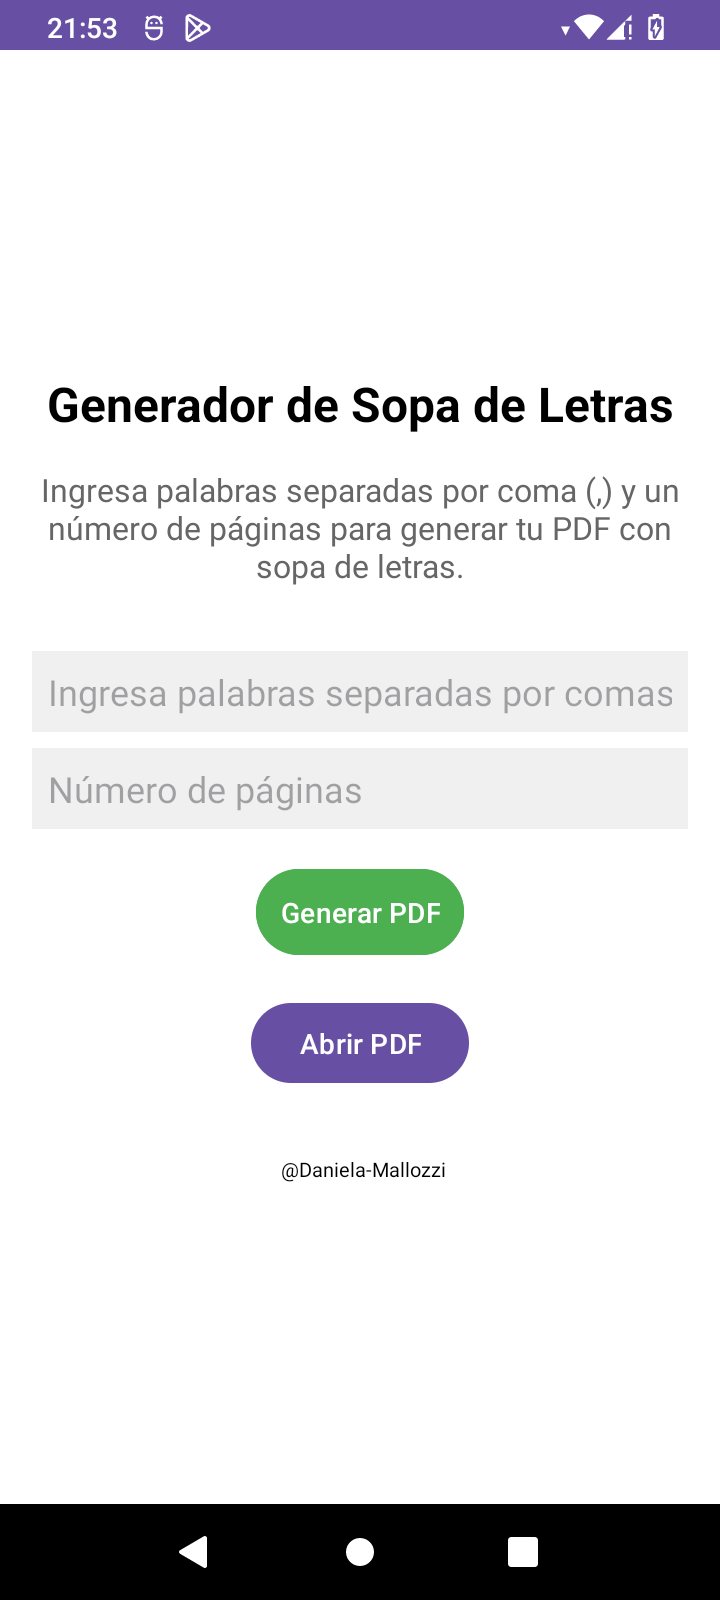
\includegraphics[width=0.6\columnwidth]{imagenes/inicio.png}
    \caption{Pantalla inicial de la app para la creación de sopa de letras.}
    \label{fig:1}
\end{figure}
Así mismo se hicieron validaciones en los botones, en el caso de que el usuario quiera presionar el botón de Generar PDF sin antes llenar los dos campos de palabras y número de página; se le presentará al usuario el mensaje de \enquote{Ingresa al menos una palabra válida} como se puede ver en la parte inferior de la Figura \ref{fig:2}.

\begin{figure}[H]
    \centering
    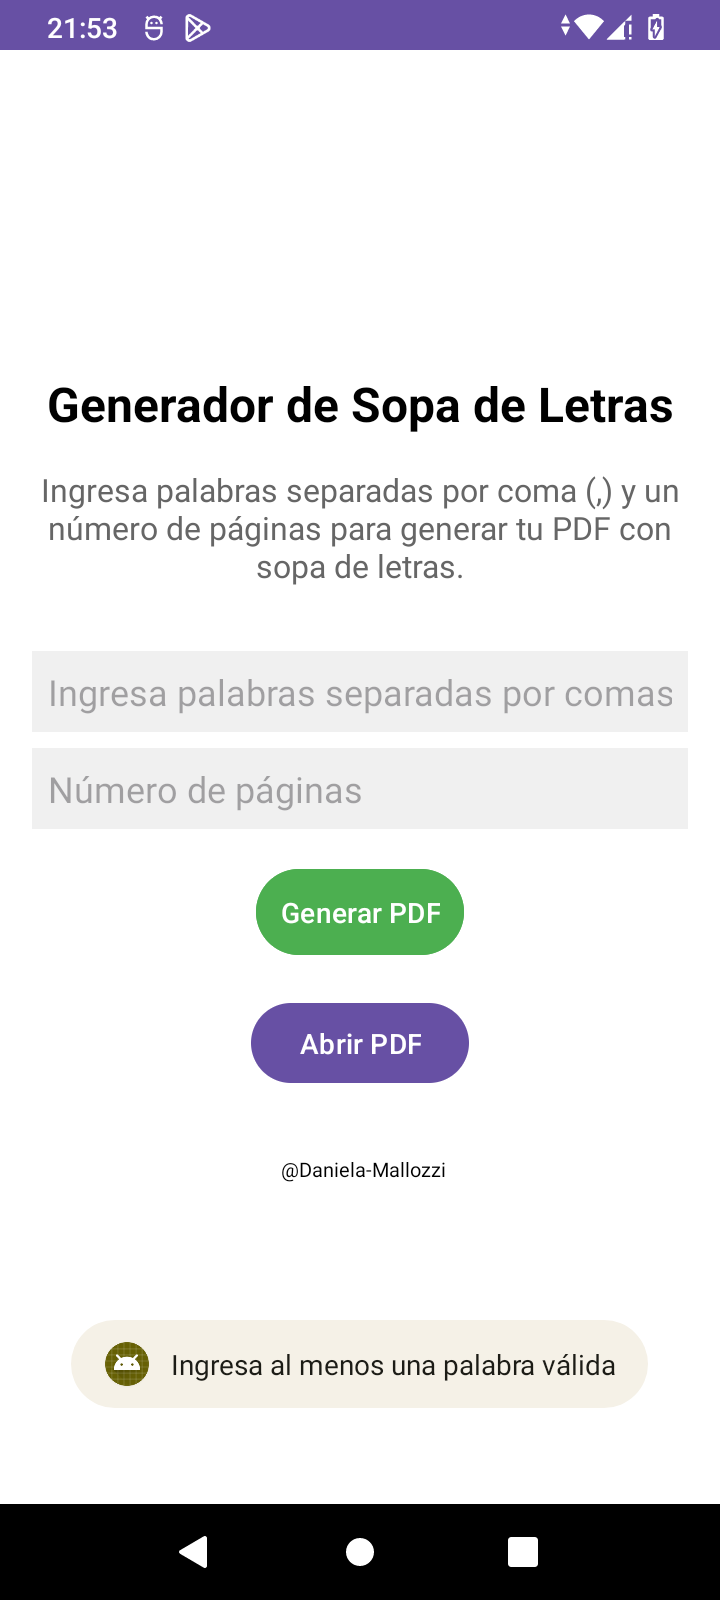
\includegraphics[width=0.4\columnwidth]{imagenes/validacion_btn1.png}
    \caption{Mensaje de validación si el usuario no ha llenado los dos campos y da click en Generar PDF.}
    \label{fig:2}
\end{figure}

De igual manera, en el caso de que el usuario solo haya llenado el primer campo de información requerida que es el de ingresar palabras y no llena el campo de número de páginas, al este hacer click en el botón Generar PDF, se le mostrará el mensaje de  \enquote{Ingresa un número válido de páginas} como se puede ver en la parte inferior de la Figura \ref{fig:3}.

\begin{figure}[H]
    \centering
    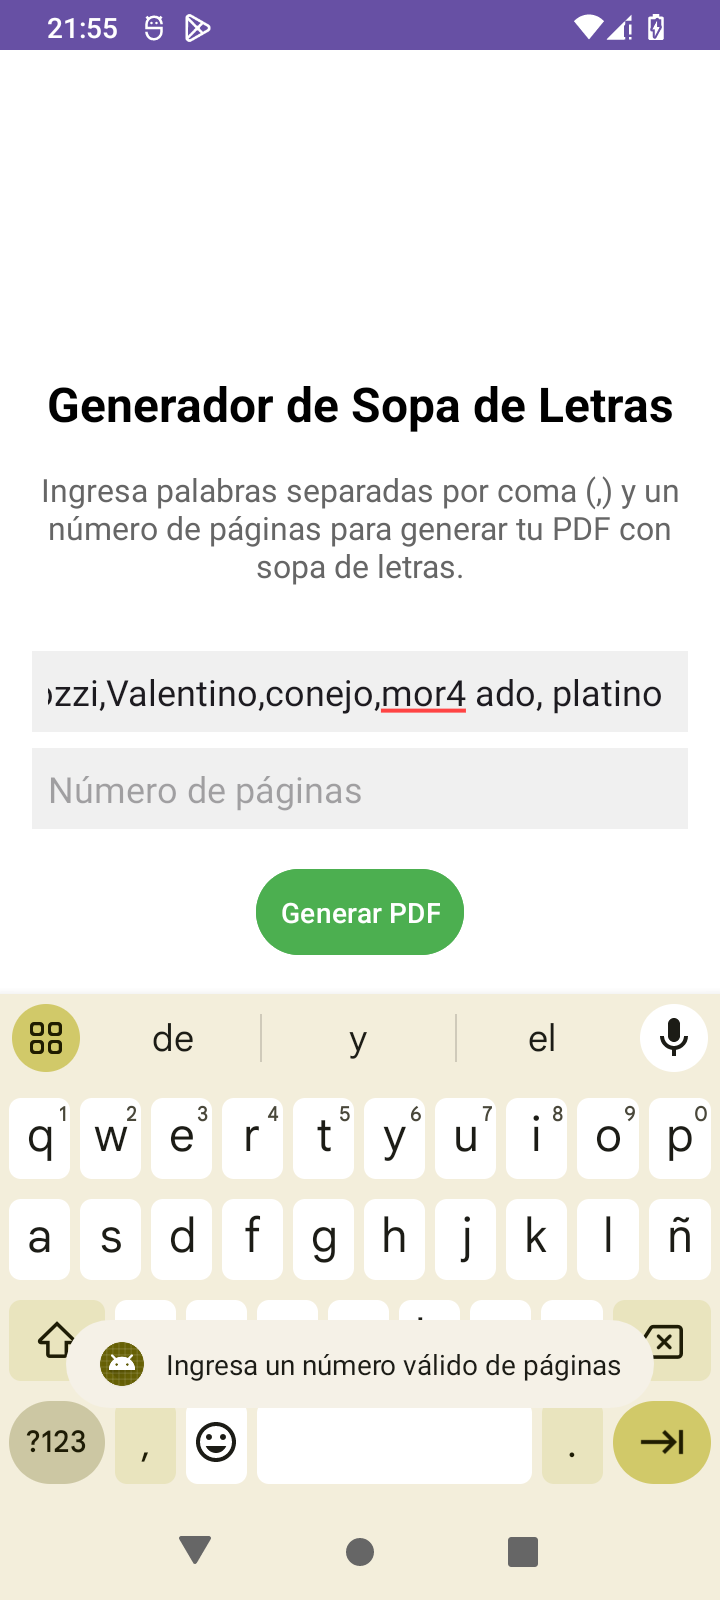
\includegraphics[width=0.4\columnwidth]{imagenes/validacion_btn1_2.png}
    \caption{Mensaje de validación si el usuario no ha llenado el campo de número de páginas y da click en Generar PDF.}
    \label{fig:3}
\end{figure}

También se cuenta con la válidación del botón de Abrir PDF, el cual mostrará un mensaje en pantalla de \enquote{Genera un PDF con tu sopa de letras primero. El PDF no se ha encontrado} como lo podemos apreciar en la figura \ref{fig:4}, si el usuario presiona el botón de Abrir PDF sin antes haber generado PDF alguno, es decir que no haya hecho el proceso de llenado de los campos para la sopa de letras. Así que, el usuario no podrá tener la funcionalidad de Abrir PDF sin antes haber generado su PDF.
\begin{figure}[H]
    \centering
    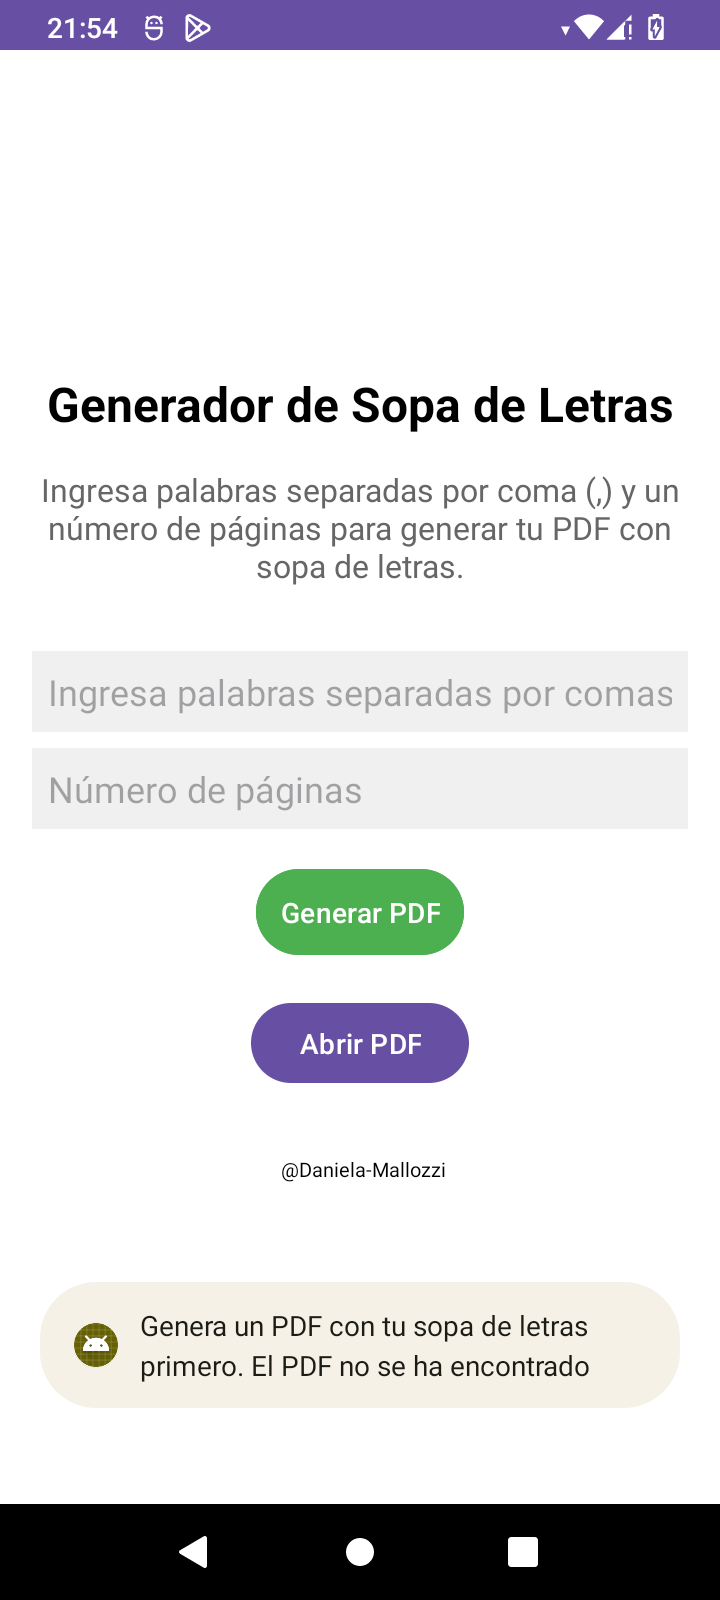
\includegraphics[width=0.4\columnwidth]{imagenes/validacion_btn2.png}
    \caption{Mensaje de validación si el usuario presiona el botón de Abrir PDF sin haber generado la sopa de letras antes.}
    \label{fig:4}
\end{figure}



Con todo lo anterior mencionado, un ejemplo correcto de llenado de información en los dos campos necesarios para la generación de sopa de letras, lo podemos apreciar en la figura \ref{fig:5}. 
En el cual se ingresó exactamente las siguientes palabras separadas con comas:  \enquote{daniela,mallozzi,Valentino,conejo,mor4 ado, platino} y se seleccionó 5 como número de páginas.

La aplicación valida diferentes casos de llenado de datos; si el usuario escribe palabras con espacio, el sistema elimina y junta las letras para así formar una sola palabra. También si se ingresan números el sistema los descarta y une las palabras sin tomar en cuenta el número ingresado. Así mismo el sistema convierte las letras ingresadas a mayúsculas para mejor legibilidad en la sopa de letras.
\begin{figure}[H]
    \centering
    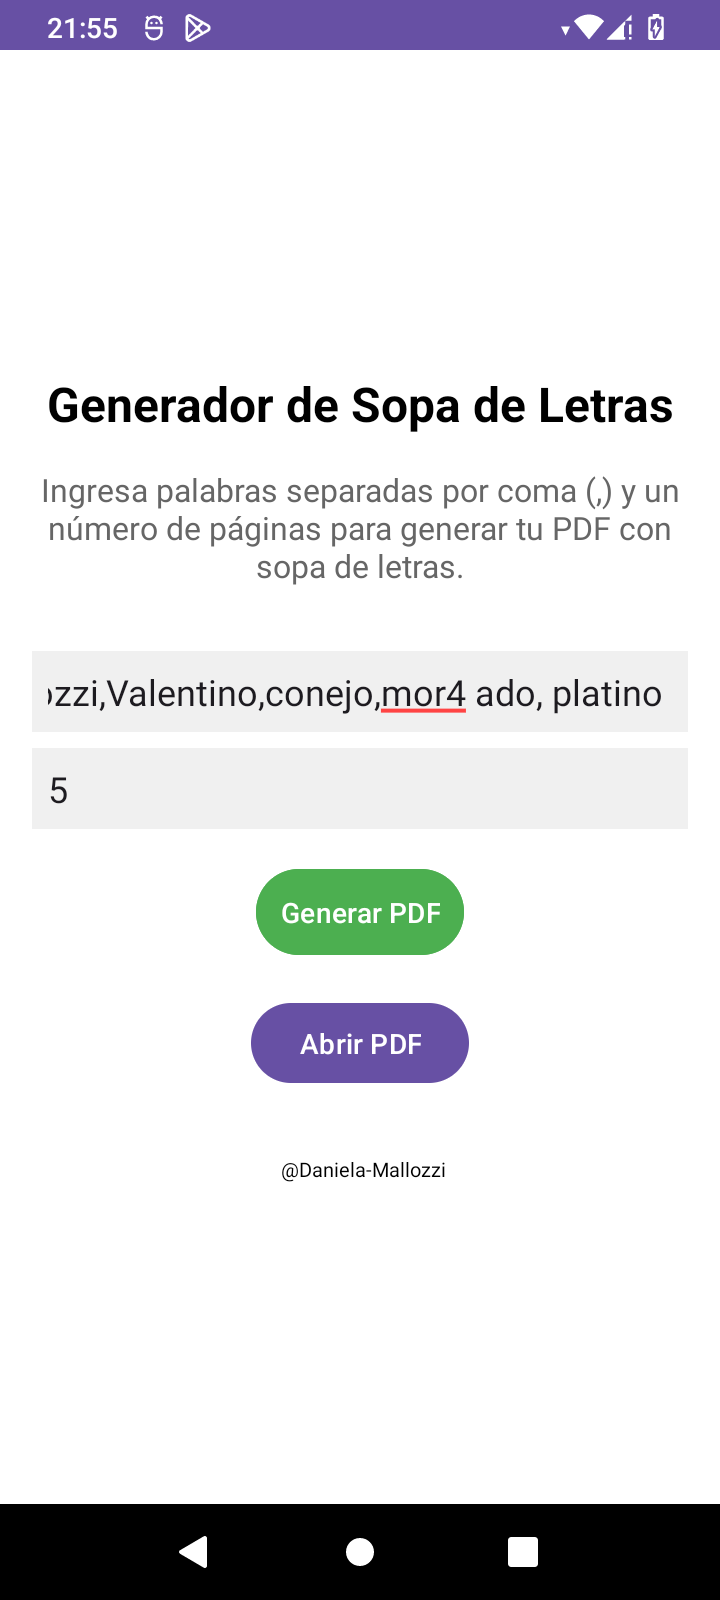
\includegraphics[width=0.4\columnwidth]{imagenes/datos.png}
    \caption{Ejemplo de llenado correcto de datos en los campos.}
    \label{fig:5}
\end{figure}



Después de llenar los dos campos de datos necesarios, el usuario puede proceder a presionar el botón Generar PDF, en la figura \ref{fig:6} se aprecia un mensaje de confirmación de PDF generado.

\begin{figure}[H]
    \centering
    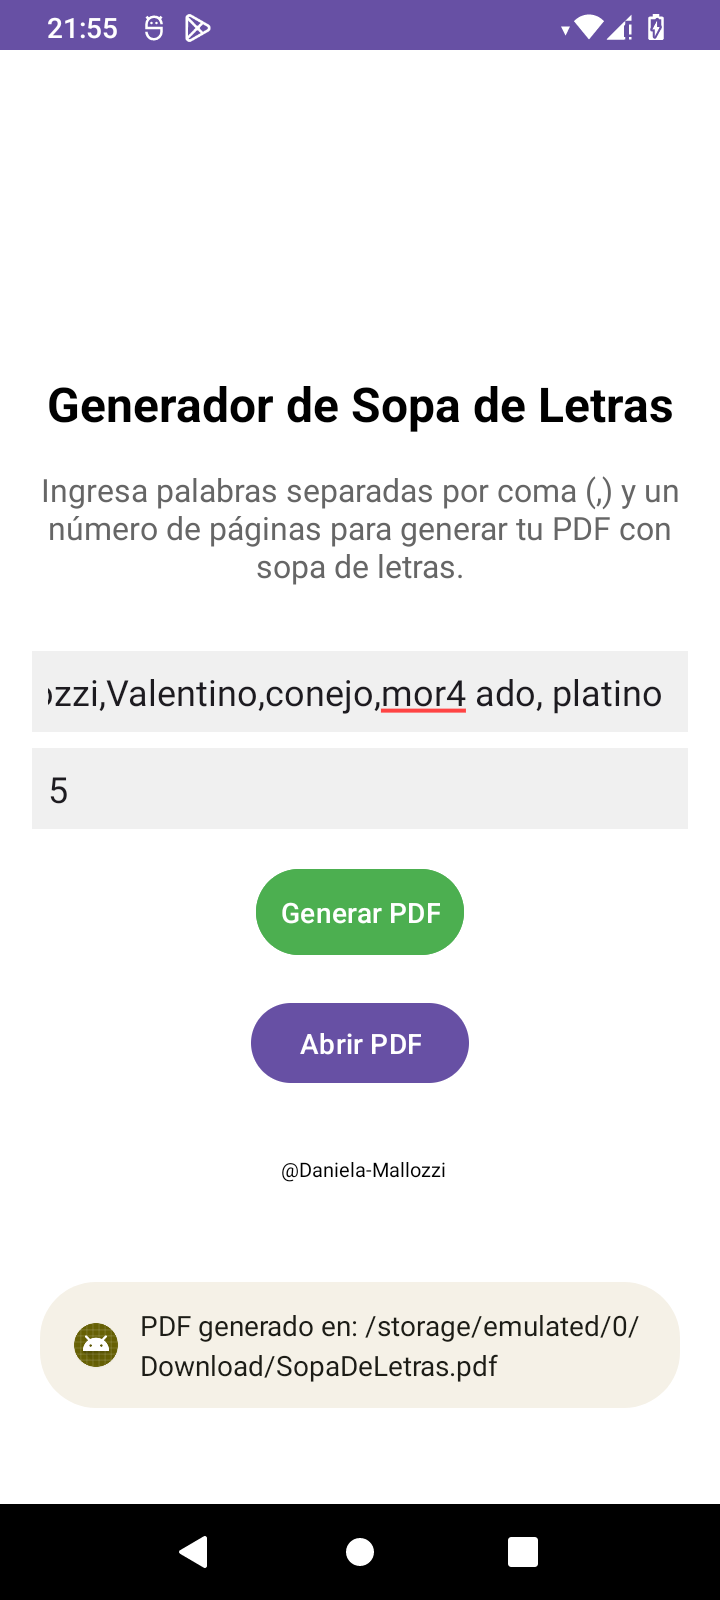
\includegraphics[width=0.4\columnwidth]{imagenes/pdf_hecho.png}
    \caption{Mensaje de confirmación al presionar botón de Generar PDF.}
    \label{fig:6}
\end{figure}


Después de haber generado el PDF, el usuario podrá hacer click en el botón Abrir PDF, para que pueda visualizar su sopa de letras personalizado. En el archivo PDF podrá encontrar la sopa o sopas de letras como se puede ver en la figura \ref{fig:7}, al inicio de cada página se mostrará el número de sopa de letras y las palabras a buscar, todo esto previamente seleccionado por el usuario, por cada página se verá una sopa de letras de diferente manera pero con las mismas palabras a encontrar, esto se genera de manera aleatoria.

\begin{figure}[H]
    \centering
    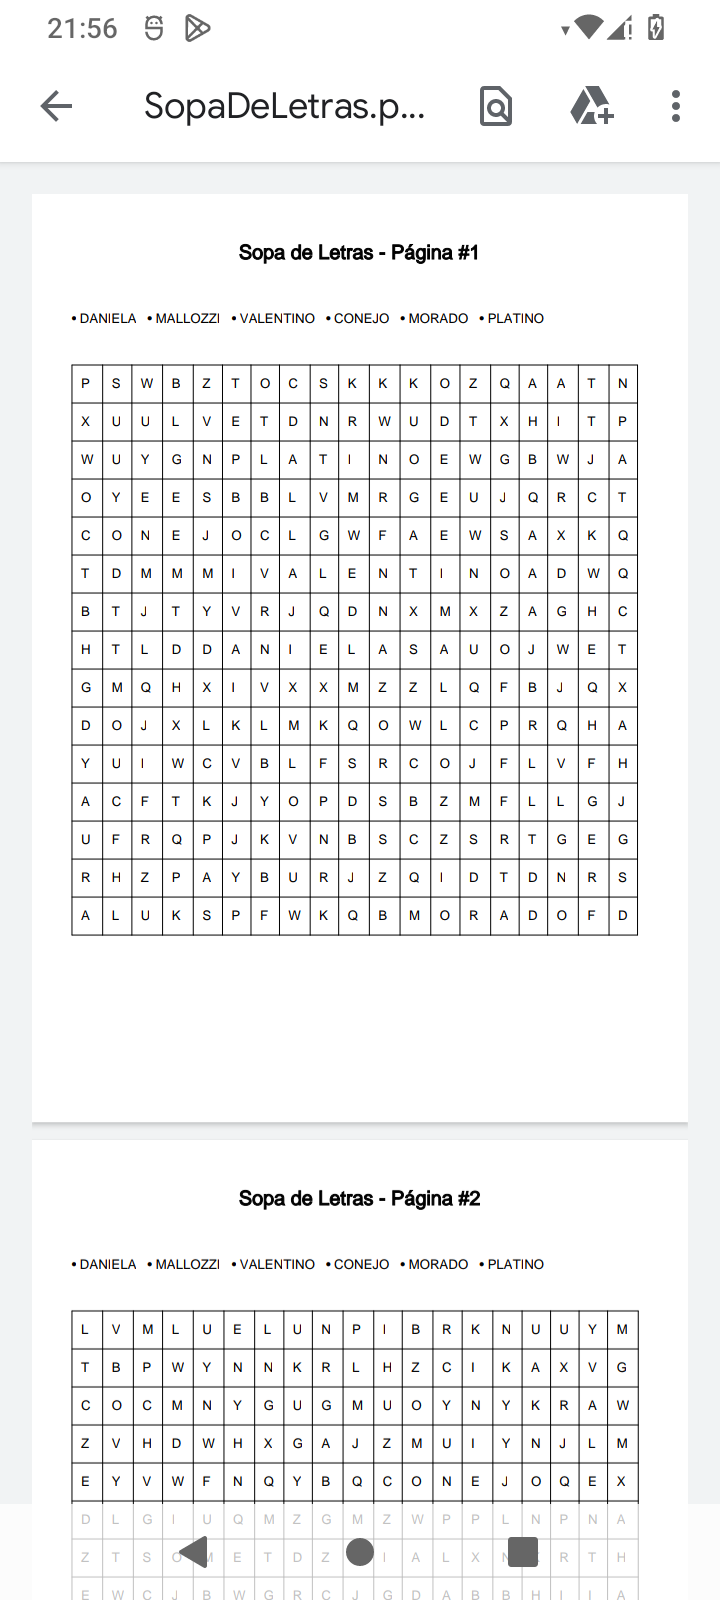
\includegraphics[width=0.4\columnwidth]{imagenes/ver_pdf.png}
    \caption{Archivo PDF con sopa de letras generado.}
    \label{fig:7}
\end{figure}


Sigueindo el ejemplo dado, se generaron 5 sopas de letras aleatorios pero con las mimsmas palabras a buscar las cuales son: \enquote{DANIELA, MALLOZZI, VALENTINO, CONEJO, MORADO Y PLATINO}. En la figura \ref{fig:8} se presenta la sopa de letras número 2 generada por la aplicación, y en la figura \ref{fig:9}  se muestra la resolución de esta para demostrar que se pueden encontrar las palabras clave ingresadas por el  usuario.


\begin{figure}[H]
    \centering
    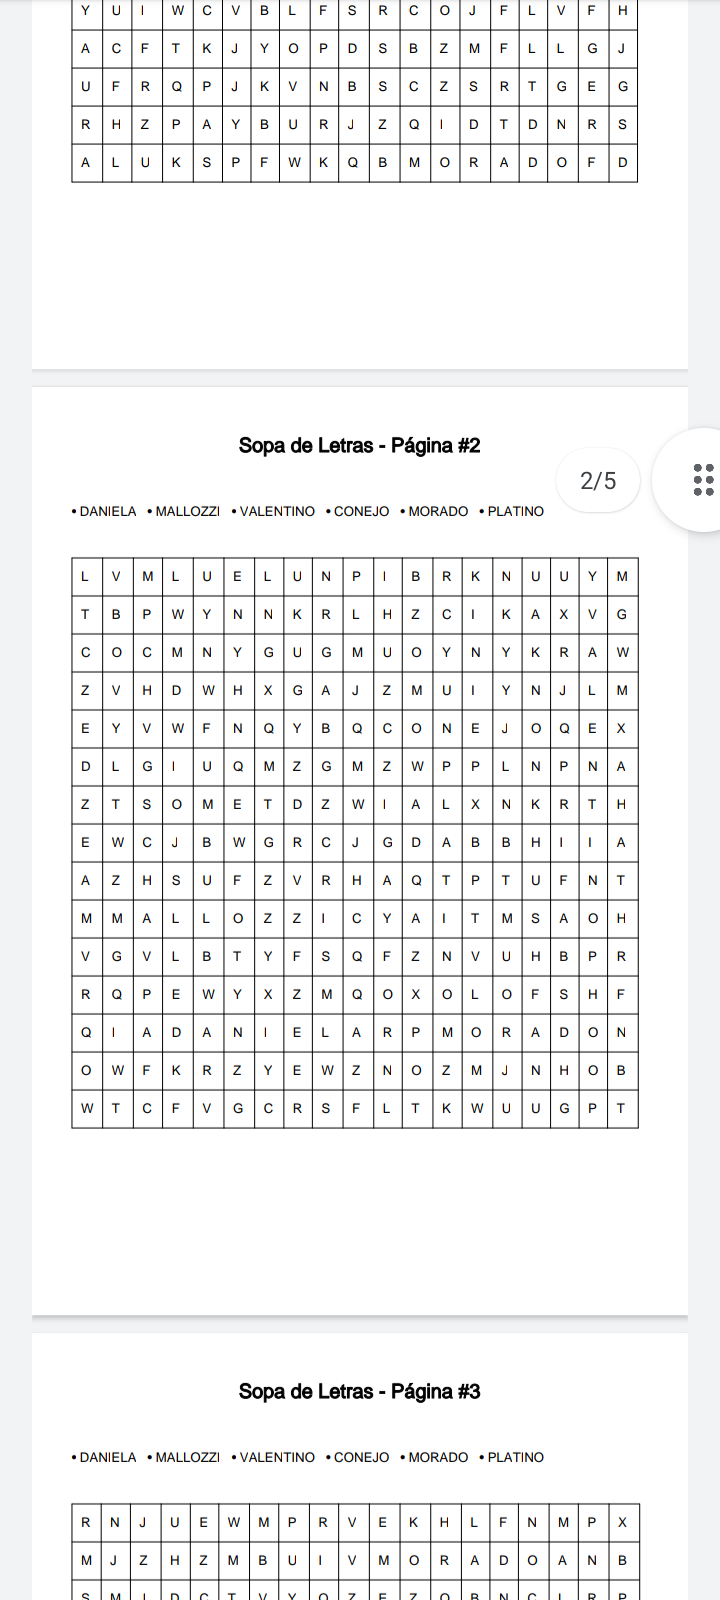
\includegraphics[width=0.4\columnwidth]{imagenes/ver_pdf2.png}
    \caption{Página 2 de la sopa de letras personalizada.}
    \label{fig:8}
\end{figure}

\begin{figure}[H]
    \centering
    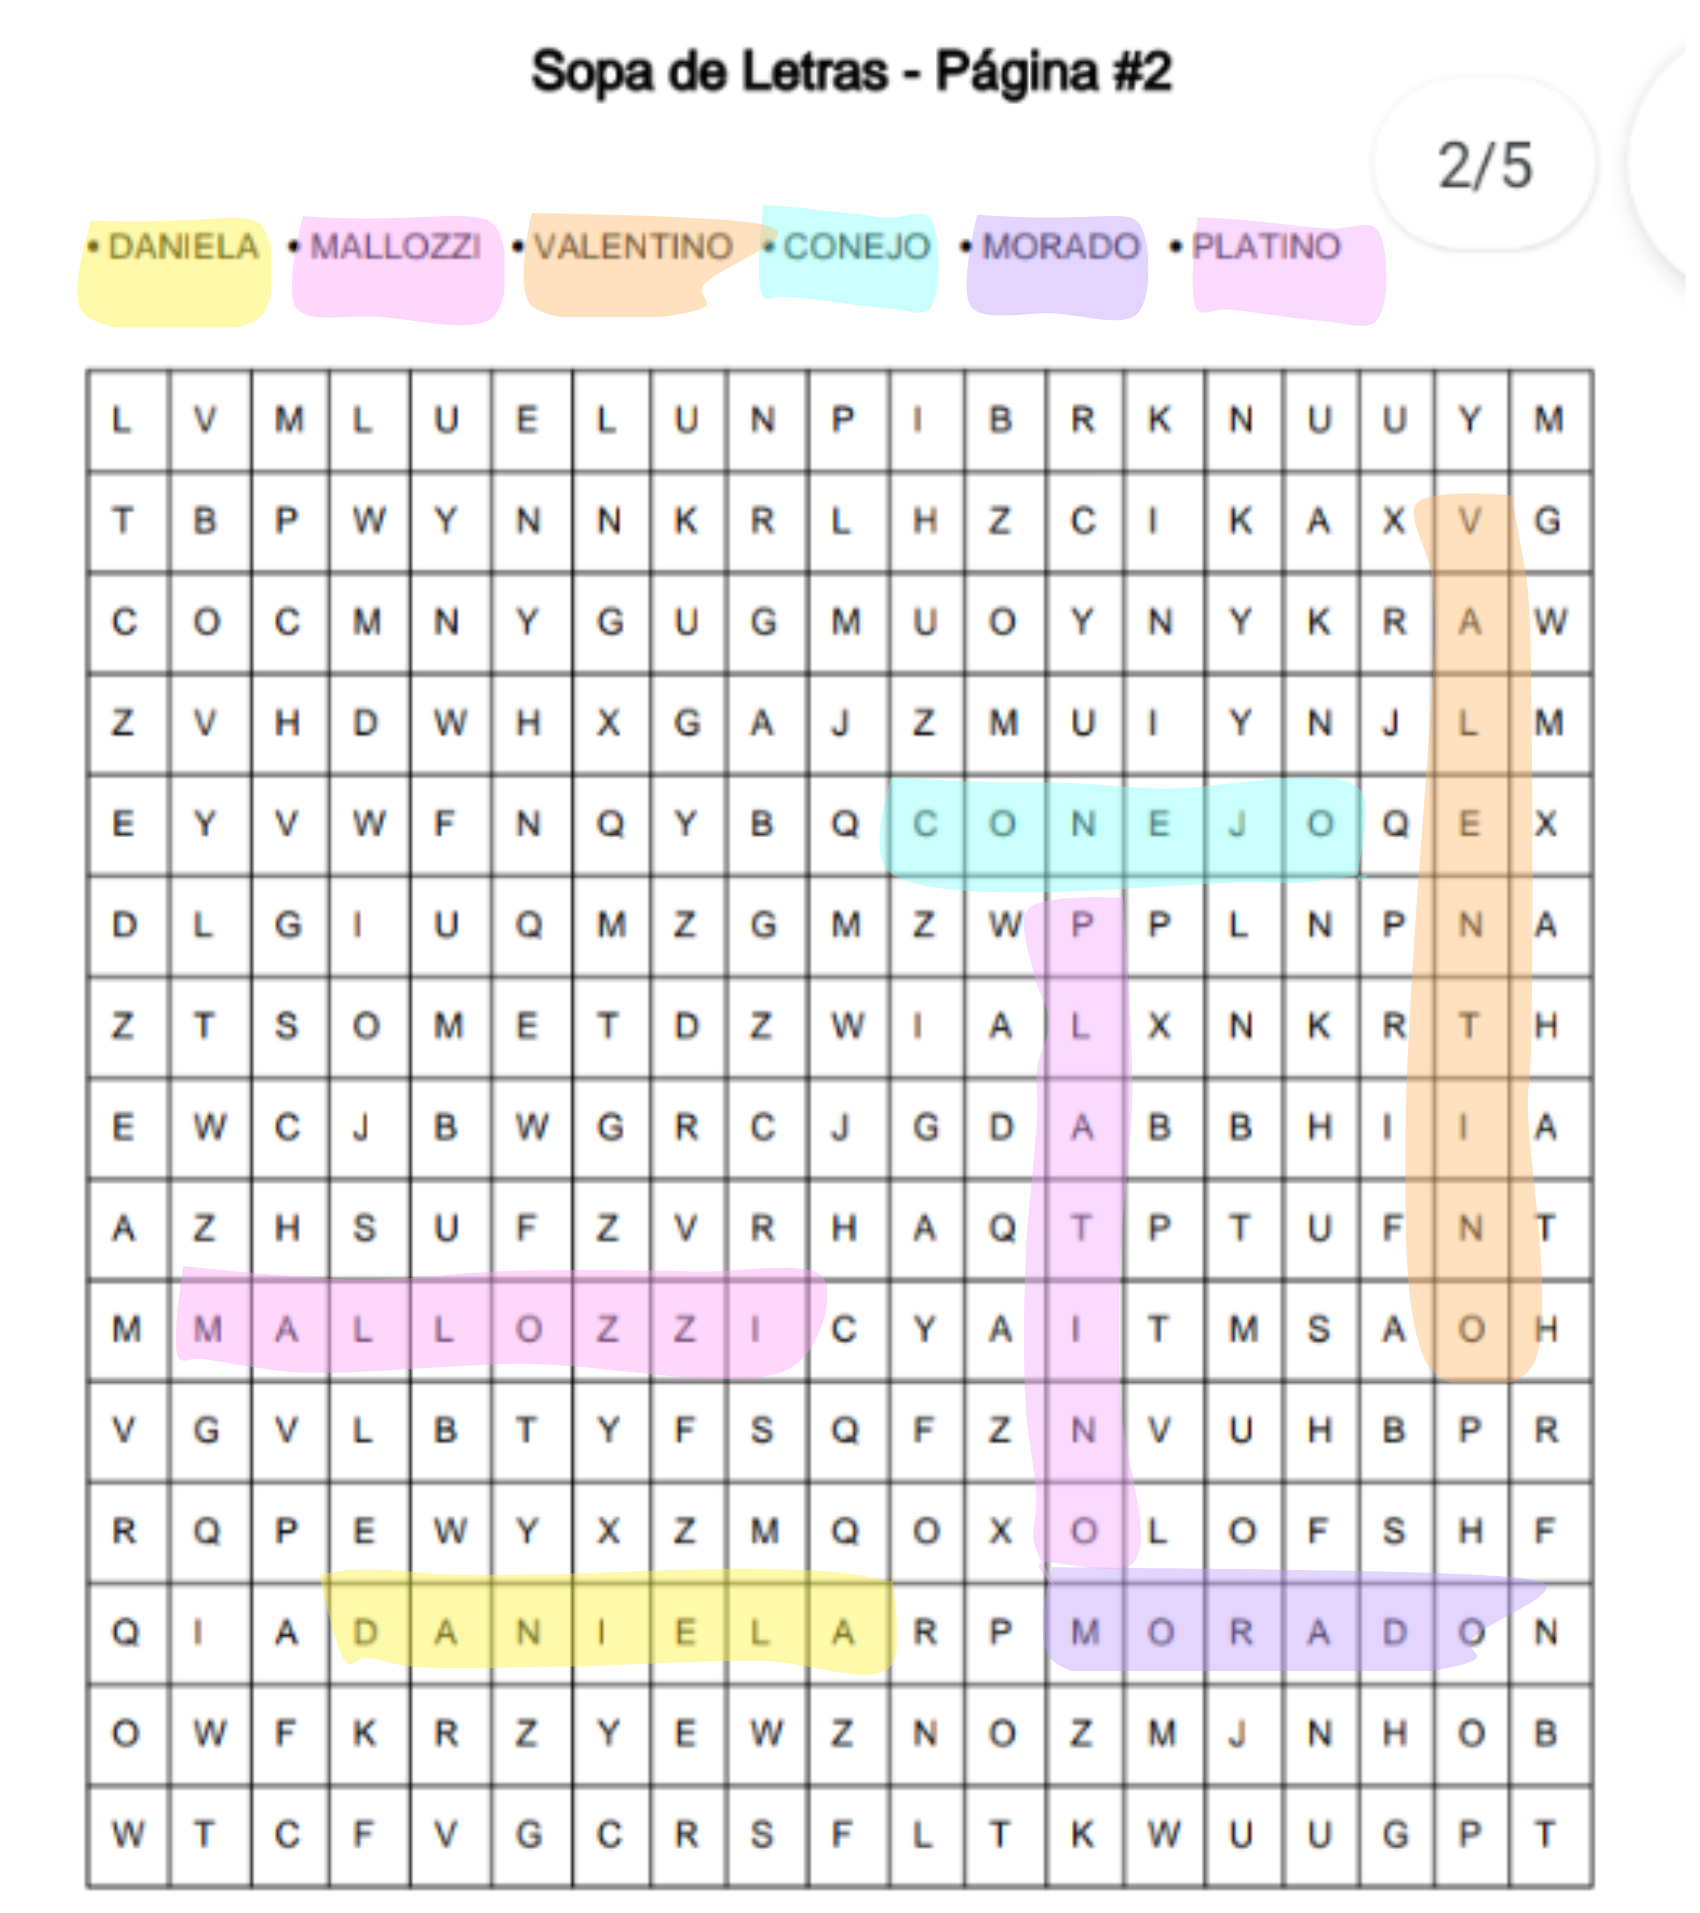
\includegraphics[width=0.9\columnwidth]{imagenes/solucion2.png}
    \caption{Resolución de la página 2 de la sopa de letras personalizada.}
    \label{fig:9}
\end{figure}


A continuación se presentan todas las páginas del archivo PDF generado con una sopa de letras hecha de manera aleatoria para que cada una sea diferente a la otra pero contanco con las mismas palabras clave. 
En la figura \ref{fig:10} se muestra la tercera página de la sopa de letras. De la misma forma en la figura \ref{fig:11} se muestra la cuarta página de la sopa de letras. Y finalmente en la figura \ref{fig:12} se muestra la quinta y última página de este ejemplo de la sopa de letras.

\begin{figure}[H]
    \centering
    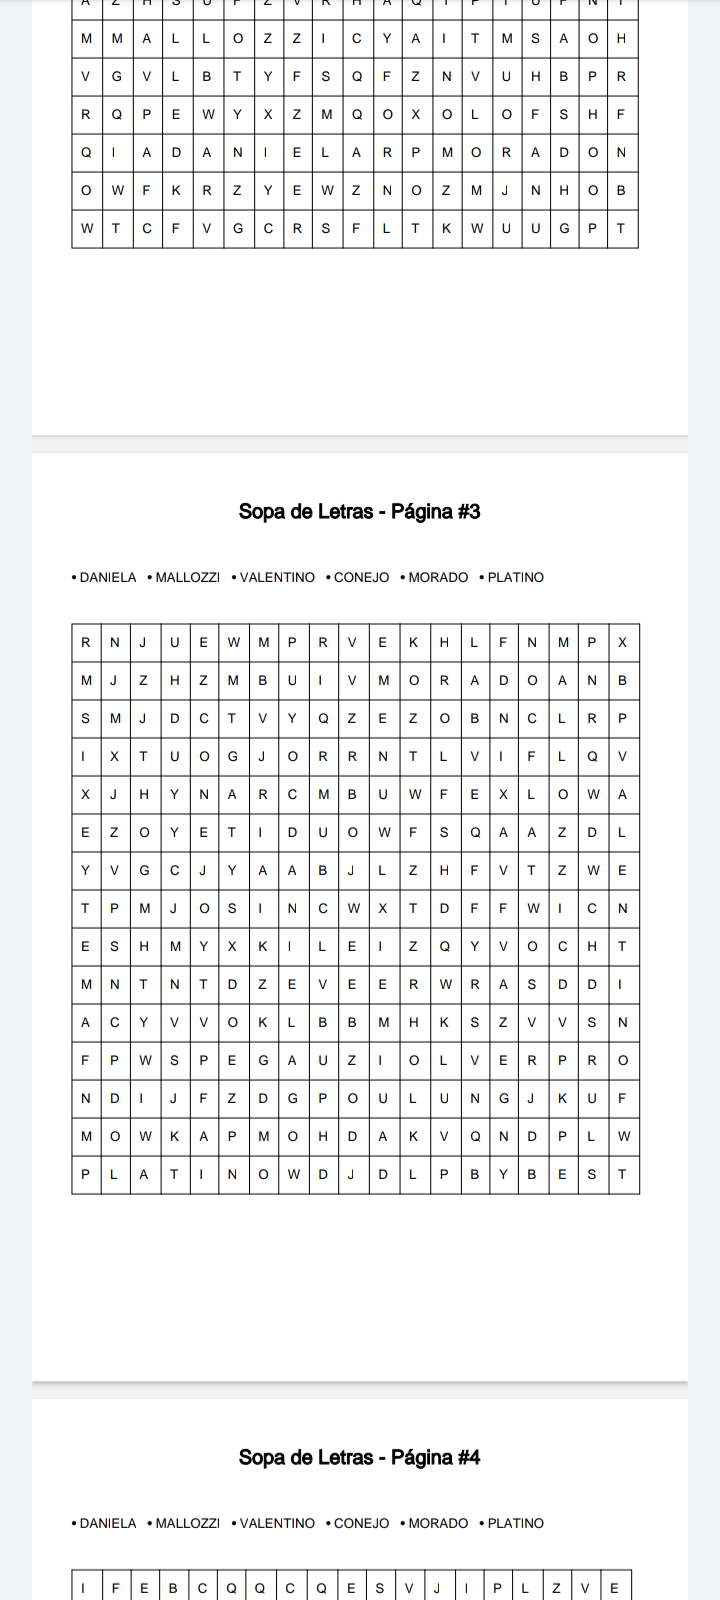
\includegraphics[width=0.4\columnwidth]{imagenes/ver_pdf3.png}
    \caption{Página 3 de la sopa de letras personalizada.}
    \label{fig:10}
\end{figure}

\begin{figure}[H]
    \centering
    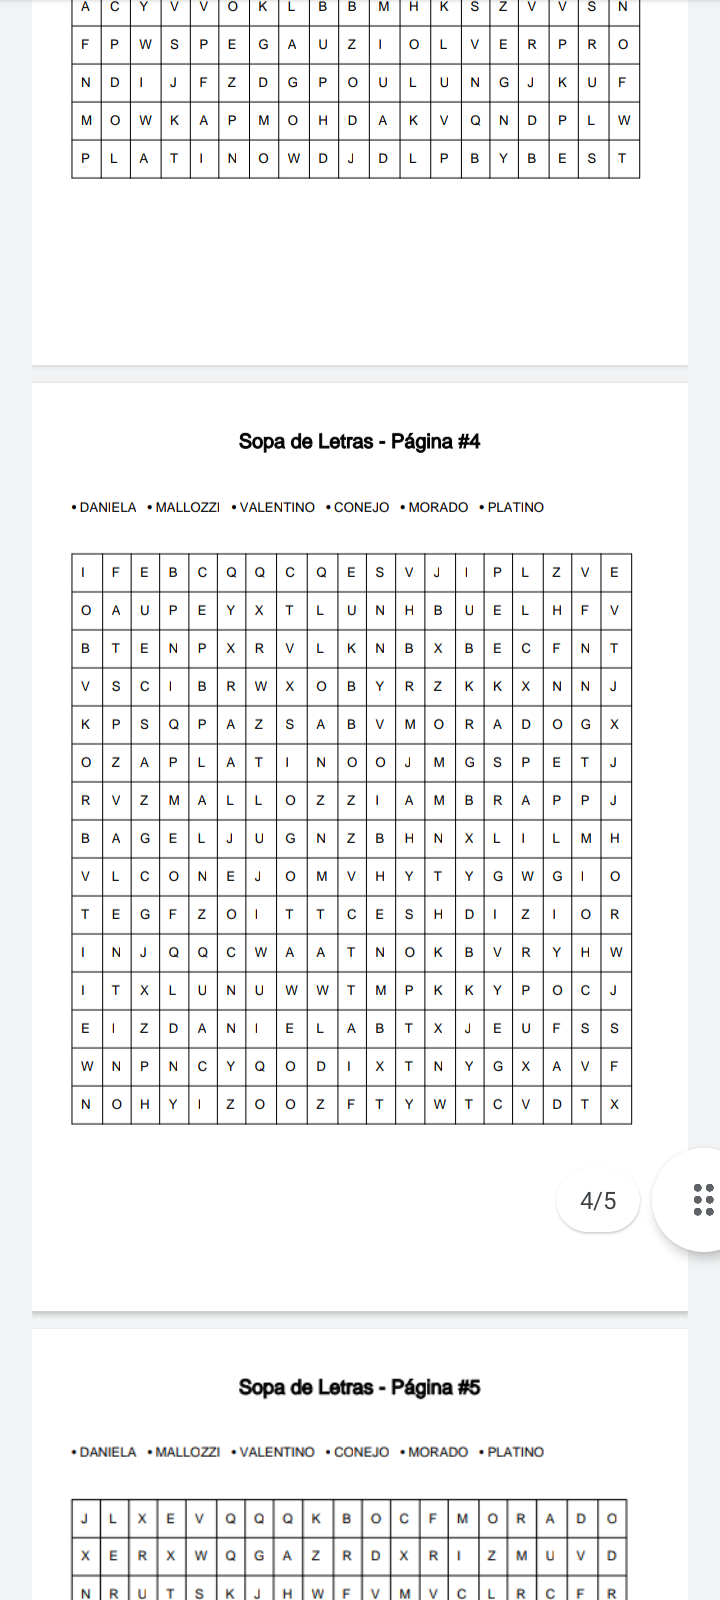
\includegraphics[width=0.4\columnwidth]{imagenes/ver_pdf4.png}
    \caption{Página 4 de la sopa de letras personalizada.}
    \label{fig:11}
\end{figure}

\begin{figure}[H]
    \centering
    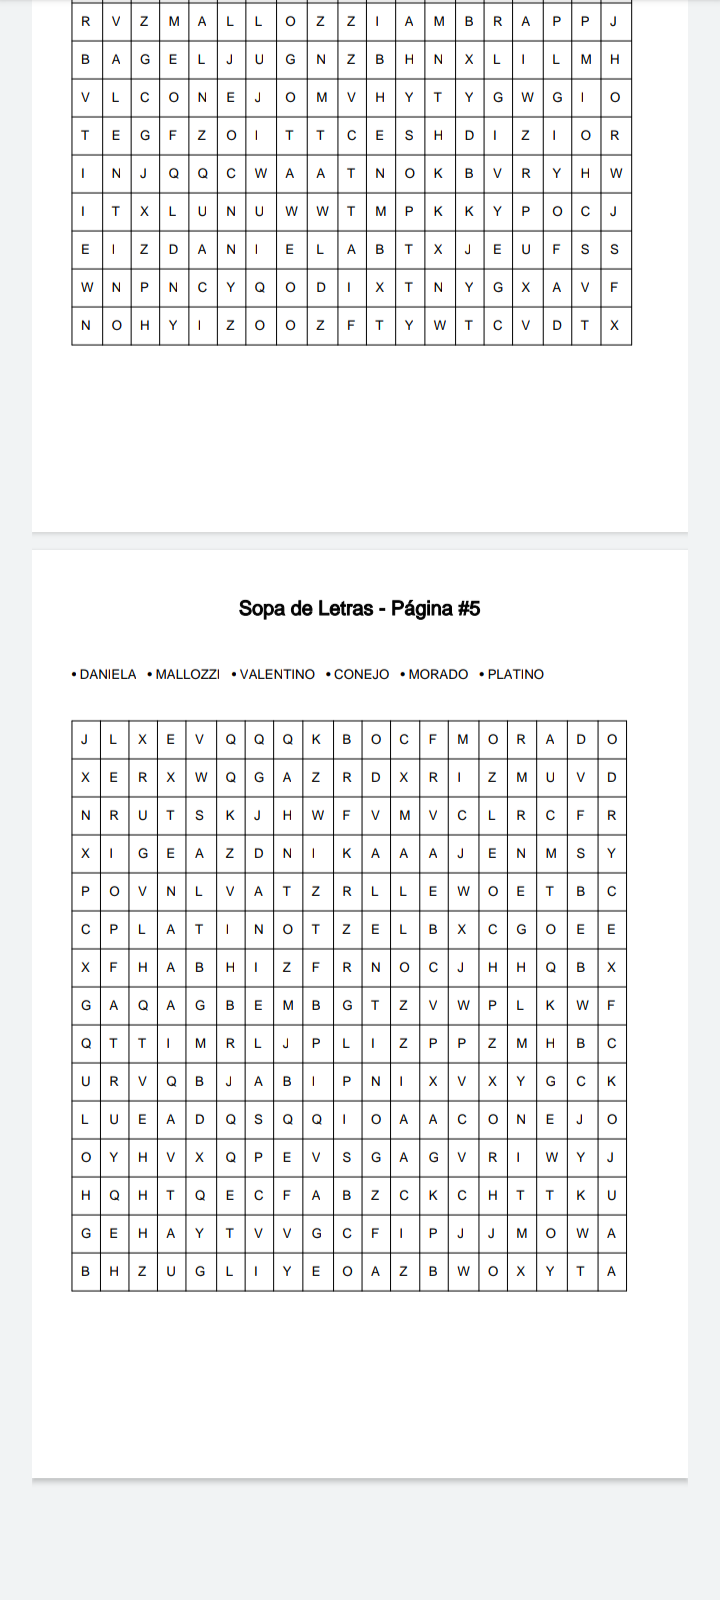
\includegraphics[width=0.4\columnwidth]{imagenes/ver_pdf5.png}
    \caption{Página 5 de la sopa de letras personalizada.}
    \label{fig:12}
\end{figure}





Como se mencionó anteriormente, el usuario tiene la opción de ver su PDF con sopa de letras mediante el botón Abrir PDF de la aplicación, pero este tambíen se puede encontrar en la carpeta de descargas de su dispositivo móvil, ver en figura \ref{fig:13}, el archivo es nombrado como \enquote{SopaDeLetras.pdf}. Cabe mencionar que cada que el usuario genere una sopa de letras diferente, el archivo se reescribirá con el mismo nombre, entonces como siempre existirá un solo archivo de tal nombre, se deberá compartir dicho archivo antes de generar otro, si así lo desea el usuario.

\begin{figure}[H]
    \centering
    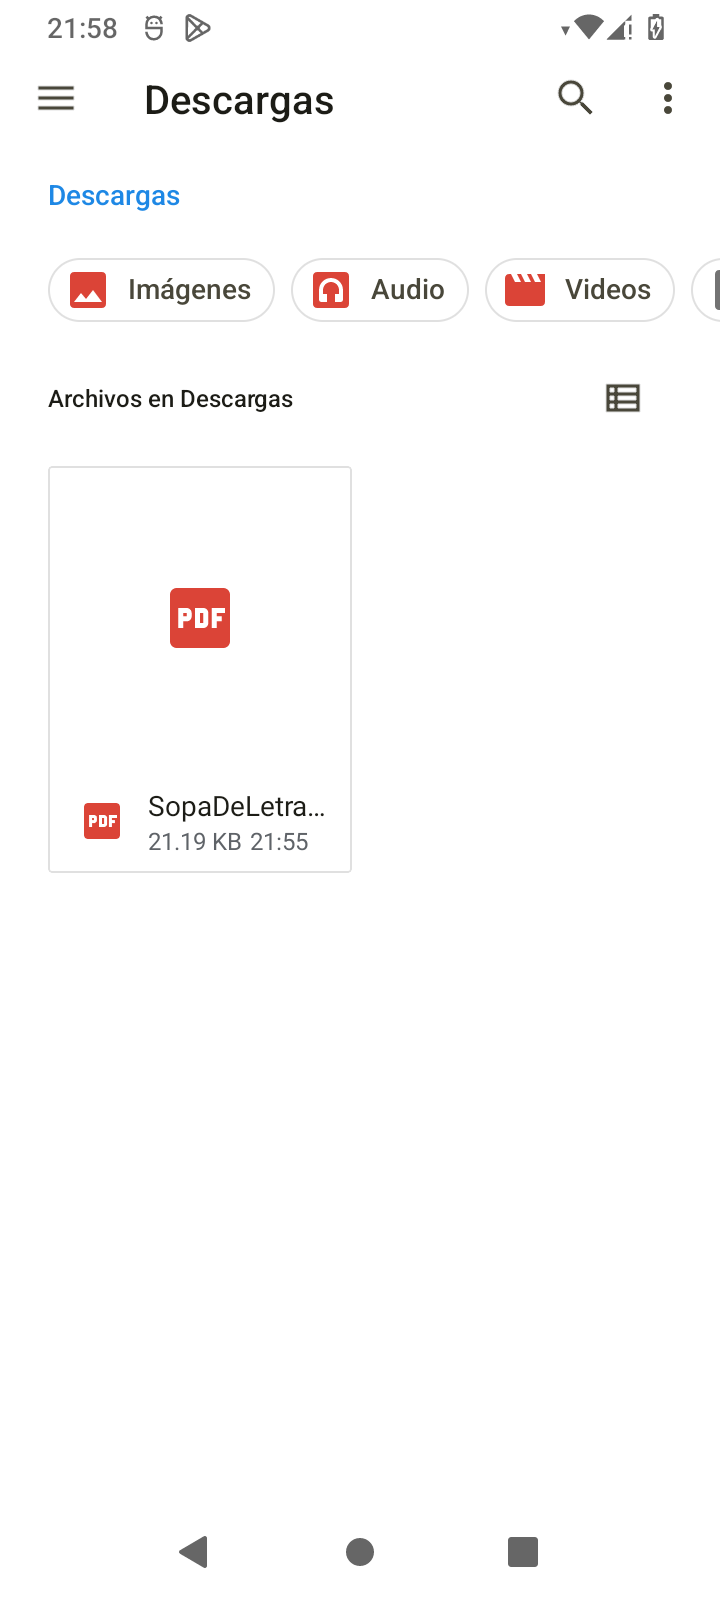
\includegraphics[width=0.6\columnwidth]{imagenes/archivo.png}
    \caption{Archivo PDF guardado en carpeta de Desacrgas del dispositivo móvil.}
    \label{fig:13}
\end{figure}





\section{Conclusión}
Este proyecto ha logrado desarrollar una aplicación móvil funcional que permite generar sopas de letras personalizadas en formato PDF. La herramienta proporciona una interfaz amigable para el usuario, y la generación del PDF se realiza de manera rápida y eficiente. El uso de Android Studio y bibliotecas como iText permitió el desarrollo de una aplicación sólida y escalable.

Se lograron características clave como permitir la personalización de las palabras, así como la elección de cuantas sopas de letras distintas se requieren, lo cual enriquece la experiencia del usuario al usar esta aplicación. Este desarrollo refuerza los conceptos fundamentales de programación en Android y la manipulación de librerías, aplicando buenas prácticas de diseño de interfaces para dispositivos móviles.

Este tipo de aplicaciones tiene un gran potencial educativo, ya que las sopas de letras pueden ser utilizadas como herramientas interactivas para mejorar el vocabulario y la comprensión de temas específicos.

\vspace{3cm}

\addcontentsline{toc}{section}{Referencias} 
\printbibliography

\end{document}
